% offset graph is caused by static friction
% inverse square relation is likely caused by ???
% I don't know what else there is to say
% oh yes, magnetic field strengh, etc etc
\section*{Discussion}

While the points on Figure \ref{fig:procplot} are visibly correlated and have a strong correlation coefficient with the plotted regression, the shape of the points suggests the current induced in the wire and the force measured are closely but not linearly related.
Given that the random error is too small to result in meaningful differences, this means that either there exists systematic error in the experiment, the hypothesis that current is linearly related to force is incorrect, 

There are a few possibilities that could have led to the deviation from the hypothesis.
Friction between the supports and the wire can explain the qualitative observation of fluctuation between currents.
In addition to the changing points of contact resulting in varying current as the pendulum swings, friction between the hooks of the wire and the hinges of the supports would create resistance torque which would set a force threshold before the wire can deflect.
While this does explain the fluctuations in current and erratic swinging, the resistance torque should not increase as the deflection angle increases.
This is because, as the deflection angle increases, the weight of the wire will become distributed between the supports and the end of the vertical length of the wire (the bottom of the wire), of which will be supported by the Lorentz force.
In addition, friction was considered in the procedure, where the hinges had to be loose enough to allow the wire to swing freely.
Given an analysis of torque on the experiment is beyond the scope of this investigation, the best guess that can be given is that friction is insignificant to the results of the experiment.

Another possibility is the experiment failed to consider the force of attraction between the supports and the wire.
Since both are conductors and have current flowing between them, they will create a magnetic field that will influence the other, hence experience attraction or repulsion between each other.
Knowing from Lorentz force, if current in one wire is going the opposite direction of current in the other wire, they will repel each other, which could attribute to a slight increase in force at lower deflection angles.
The force exerted between the two wires can be estimated by using the definition of the ampere:
``One ampere is defined as the current that would cause a force of $2 \times 10^{-7}\si{\newton}$ per metre between two long parallel conductors separated by $1\si{\meter}$ in a vacuum.''\footcite{pearsonamp}
Right away, $2 \times 10^{-7}\si{\newton}$ is three orders of magnitude below the measured force, meaning that, even with one ampere going through the wire, the contributing force would be unnoticeable.
This means the attraction between the supports and the wire is not the main cause of the deviation from a linear relation in the experiment.

Since, the horizontal segment of the wire did vary in distance between the magnets, it is possible that the B-field varied by a significant amount as the wire swung during the experiment.
Although magnetic field strength does not exactly follow the inverse square law, its strength still decreases substantially with distance.
At the minimum and maximum deflection angles (around $5\si{\degree}$ or $30\si{\degree}$) the magnetic field could have been stronger than the rest of the angles.
However, the opposite is reflected in the data in Figure \ref{fig:procplot}, as force at the low and high currents are below the linear regression, while points in the middle are above the linear regression.
This does not mean variation in magnetic field strength is ruled out.
There is the possibility that, despite using large magnets, the magnetic field between the two magnets was not uniform.
Using the magnetic gap calculator from K{\&}J Magnetics, the magnetic field strength relative to the distance from the center axis between two cylindrical magnets can be determined.\footcite{kjgap}
By approximating the dimensions of the experiment magnets as cylindrical magnets, the graph in Figure \ref{fig:gaps} was produced.
\begin{figure}[H]
	\centering
	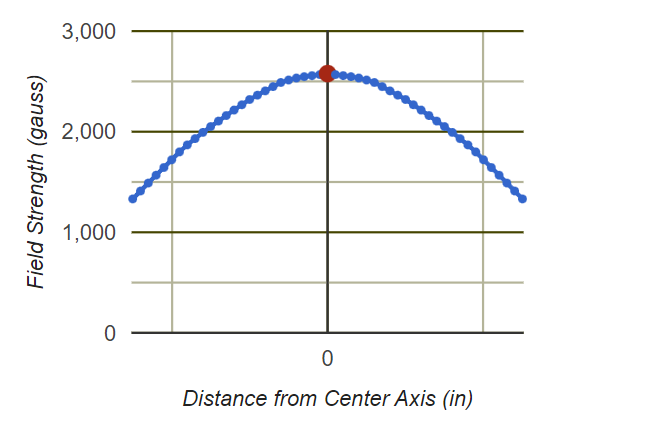
\includegraphics[width=0.5\textwidth]{figures/gapplot.PNG}
	\caption{Distribution of field strength over distance from the center axis between two magnets.}
	\label{fig:gaps}
\end{figure}
This would explain why the force at the minimum and maximum angles varies from a linear relation; the magnetic field strength decreases when the wire is further away from the center.

